\chapter{\protect Methods}

\section{Laboratory Astrophysics}
To study the chemical reactivity in astrophysical environment experimentally,
we conducted our experiments in Interstellar photoprocessing system (IPS) (Chen et al. 2014),
an ultrahigh vacuum chamber with base pressure $3 \times 10^{-10}$ torr and 14 K,
corresponds to a density of $10^6$ cm$^{-3}$, similar to dense cloud interiors.
The system will be introduced in detail in section \ref{sec:IPS_system}.
To simulate the irradiation in interstellar environments,
we use a micro-wave discharge hydrogen lamp (MDHL) and monochromatic extreme-ultraviolet irradiation (EUV) 30.4 nm to irradiate our ice mixtures,
and they will be introduced in section \ref{sec:Vacuum_UV_source} and \ref{sec:Extreme_EUV_source} respectively.
The experimental protocols will be elaborated in section \ref{sec:Experimental_Protocol}.
In order to better understand the physics behind, some basic theories of Infrared spectroscopy and concepts of chemical kinetics used in data analysis are included in section \ref{sec:spectroscopy} and \ref{sec:Reaction_Rate_Laws} respectively.
To demonstrate the ice mixtures in KBOs, we used different configurations of ice mixtures that refers to different sections in chapter 3 and chapter 4.\\

\subsection{Experimental simulations by IPS system}
\label{sec:IPS_system}

We conducted our astrophysical simulations studied in chapter 3 to 4 in Interstellar Photo Processing System (IPS) (figure \ref{fig:system}). IPS consists in three systems: the main chamber, where our experiments take places; the detection system, where we collect our data; and a gasline system, where we prepare our samples.

\begin{figure}
\centering
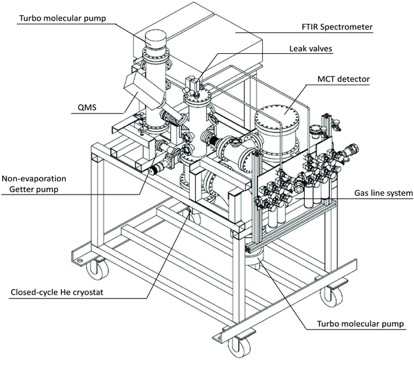
\includegraphics[width=\textwidth]{figures/chapter2/system.jpg}
\caption{The schematic diagram of IPS system, mechanical pumps are not shown for clarity. (Quoted from Chen et al. 2014)}
\label{fig:system}
\end{figure}

The main system consists of an ultrahigh vacuum chamber equipped with a closed-cycle helium cryostat (CTI-M350). It is pumped by a turbo molecular pump (KTKT FF – 160/620ZE, capacity 600 liters s$^{-1}$), which is backed up by a scroll pump, and a non –evaporation getter pump. The getter pump is a powerful tool to adsorb residue gases inside the main chamber, with a larger surface area, H$_2$, CO and N$_2$ are adsorbed to obtain a better base pressure. After baking, the base pressure of our main chamber can reach $1 \times 10^{-10}$ torr at 14 K, monitored by a Granville-Phillips 370 Stabil-Ion gauge. This pressure can be used to demonstrate the dense cloud interior environments and star forming region. The substrate we have chosen is KBr, which can allow infra-red photons with 700 to 4000 $cm^{-1}$ to penetrate. It is mounted by substrate holder made of oxygen-free copper, on the first stage of cold finger mounted on the tip of cryostat. Two silicon diodes and also a heater were placed onto the cold finger and one of the silicon diodes is near the substrate holder. They were connected to a temperature controller and PID system to achieve a warmup rate of 1K/min with an accuracy of 0.1 K.

The detection system consists in a mid-infrared Fourier transform spectrometer (mid-FTIR) (ABB FTLA2000-104) and a Quadrupole Mass Spectrometer (QMS). To prevent absorption bands of CO, CO$_2$ and H$_2$O gas in the atmosphere, the IR beam path was built inside vacuum, pumped by dry pump. The main chamber and the IR path are separated by ZnSe windows, which can allow infra-red penetration from 0.5 – 20 um with absorption less than 0.07 \%. In this study, the infrared spectra are obtained with resolution of 4 cm$^{-1}$ and averaged over 32 scans. The angle between the IR beam path and the substrate holder is 45 degrees. The QMS (MKS Microvision 2) consists of a controller and mechanical part sealed by a mounting flange in ultrahigh vacuum. It is mounted 10 cm from the substrate and run with a resolution 0.5 a.m.u. The Ionizer release 70 eV electron by filament and ionize incoming molecules to positive charged ions between anode grid and repeller. The ions were accelerated by focus plate and enters ion filter, which consists of four circular rods, with a combination of A.C and D.C. potential to sieve whole bandpass ions at millisecond timescale. The selected ions enter ion detector and are detected by either faraday cup and continuous dynode electron multiplier (CDEM) which can secondary multiply weak signals.

The samples are prepared in situ in our gasline system. It contains four stainless steel bottles with the same volume, which is used to determine relative proportion of the gas mixtures by their partial pressures. The ammonia gas 99.99 \% and methane 99.999 \% are mixed with partial pressure measured by a Baratron with 0 - 100 torr range with a 0.25% accuracy. The background pressure of the gasline system is lower than $1 \times 10^{-7}$ torr thank to a turbo molecular pump (Oerlikon Leybold TurboVac 151, capacity 145 liters s-1) backed up with an oil-sealed mechanical pump (Alcatel 2012A, capacity 450 $liters minute^{-1}$), equipped with an oil trap (molecular sieve type 13X). Water were bought from Merck which is LC-MS Grade and purified before use, by several freeze-pump-thaw cycles under vacuum.

\subsection{Vacuum-UV source}
\label{sec:Vacuum_UV_source}

In order to simulate the photoprocessing of vacuum ultraviolet (VUV) irradiation onto the interstellar ices and ices on planetary bodies, including KBOs, the ice mixtures are irradiated with a T-type Microwave-Discharged Hydrogen-flow lamp (MDHL). The molecular hydrogen with pressure 0.4 torr flows through the lamp with a support of a mechanical pump. Using a 2.4 GHz microwave generator and high voltage discharge, a low pressure plasma is produced in the Evenson cavity. Figure \ref{fig:T_type} shows a cross-section of T-type quartz tube; the middle part of the T-type quartz tube is being tunned by a ceramic rod that is called Evenson cavity.
\begin{figure}
\centering
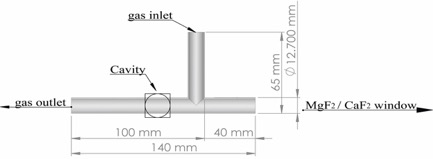
\includegraphics[width=\textwidth]{figures/chapter2/T_type.jpg}
\caption{The cross-section of MDHL (T-type geometry) (Quoted from Chen et al. 2014).}
\label{fig:T_type}
\end{figure}
In order to measure the photon flux in situ, we use an 88 \% transmittance nickel mesh with its photoelectric efficiency being obtained by high-flux beamline in National Synchrotron and a SXUV 100 photodiode calibrated by NIST. A MgF$_2$ window is placed between the lamp and the sample holder to prevent penetration of VUV photons with wavelength shorter than 114nm, leads to a cut off at 114nm. Figure \ref{fig:MDHL} shows a VUV emission spectrum of a MDHL.
\begin{figure}
\centering
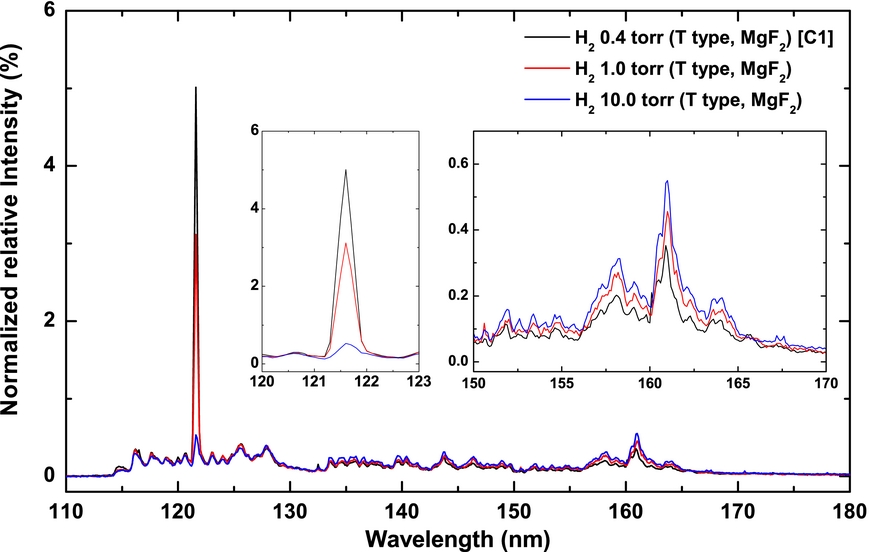
\includegraphics[width=\textwidth]{figures/chapter2/MDHL.jpg}
\caption{VUV spectra of MDHL (T-type geometry, 110-180 nm) with different H$_2$ pressure inside the lamp(Quoted from Chen et al. 2014).}
\label{fig:MDHL}
\end{figure}
It consists in Ly-α (121.6nm) and H$_2$ molecular emission in 110-180 nm range. Chen et al. (2014) showed that the spectral characteristics of the VUV light emitted in this range depends on the gas type (mixture of H$_2$ with He or Ar etc), pressure of H$_2$ and lamp geometry. Throughout those configurations stated there, we adopted 0.4 torr molecular hydrogen and T-type MDHL that produces VUV irradiation at 114-170 nm with 19.1 \% of Ly-α and a mean photon energy of 9.27 eV. The photon flux is $6.4 \times 10^{13}$ photons $cm^{-2} s^{-1}$ at sample position.

\subsection{Extreme EUV source}
\label{sec:Extreme_EUV_source}

To simulate the solar EUV irradiation reflected by IPM on both Charon and interstellar ices, we use the HF-CGM high – flux beam line of the National Synchrotron Radiation Research Center in Hsinchu, Taiwan. It provides a continuum EUV to VUV photons from 4 to 40 eV. The continuum is separated into monochromatic He II line (30.4nm) with a six-meter cylindrical grating monochrometer with an incident angle of 70 degrees. With the help of a movable entrance slit and movable curved exit slit, the energy resolving power can reach around $3 \times 10^4$ at 40 eV for grating 1600 l/mm with both slits movable and set opening to 10 $\mu m$ (Hsieh 1998). Similar to VUV irradiation provided by MDHL, the light intensity was monitored by the same nickel mesh with photoelectric efficiency obtained by SXUV 100 photodiode calibrated by NIST. With the known photoelectric efficiency, the flux of monochromatic 30.4nm is measured to be $2.15 \times 10^{14}$ photons $s^{-1} cm^{-2}$ with a spot size of 1 cm%^2% which is in the same order of magnitude of VUV continuum of MDHL. We replace the port with MDHL by the end station of the high-flux beamline. To prevent contaminations in the pipes and bellows, we placed a cryostat backed up by a scroll pump between our system and the beamline endstation. Between the cryostat and our main chamber is a SiO$_2$ valve, which is closed to prevent contamination to the end station during the warm-up phase.

\section{Experimental Protocol}
\label{sec:Experimental_Protocol}

In this section, we will briefly introduce the  procedures of how we performed our experiments. It is divided into four parts, preparation and cooling, deposition, irradiation and warmup.\\

Preparation of experiments and cooling\\
Before any of experiment is done, we bake our system at 100 oC for 48 hours to reduce the contamination of water and residue gases as much as possible. It was cooled to room temperature that the background pressure can reach routinely at $~ 1 \times 10^{-10}$ torr. The gasline were connected with the regulators of the gas tanks and bake to 100 $^oC$ and pumped by molecularturbo pump for two days before any experiment were done. Also, The water sample has been freeze thaw several times by liquid nitrogen until there is no pressure increase recorded by baratron when water is freezed. Before cooling the substrate to cryogenic temperature, we took an IR spectrum and started the monitoring of residue gases by QMS in order to compare the residue molecules and to verify any possible contaminations in the main chamber. We then start the cooling process thanks to the closed-cycle He cryostat.\\

Deposition\\
The gas mixtures are pre-mixed in our gasline system introduced in section \ref{sec:IPS_system}. We used a leak valve to condense the gas from the stainless steel bottles onto pre-cooled KBr substrate at 14 K, which monitored by Fourier transformed Infra-red spectroscopy (FTIR) and Quadrupole mass spectrometer (QMS) during deposition. The pressure of deposition is fixed to $1 \times 10^{-8}$ torr that the deposition rate is $4 \times 10^{16} molecules cm^{-2} min^{-1}$. After deposition, we placed the ice mixture at 14 K for 60 minutes and to allow pumping of residue gas, until pressure of the main chamber reduce back to its base pressure to simulate the interstellar environment before irradiation.\\

Photon Irradiation\\
The total irradiation time is 270 to 450 minutes depend on experiment configurations; with time intervals varies from 2 to 30 minutes. After each irradiation, we waited for 10 minutes allowing pumping out of the photodesorpted gas molecules. During irradiation, the photon flux is monitored by a nickel mesh. After Irradiation, we place the sample for 30 minutes to observe if any thermal reaction was conducted.\\

Warmup\\
We use 1 K/min to warmup the substrate to 300 K to demonstrate effects of a new born star nearby an interstellar cloud. During warmup, we record the QMS from 1 to 100 a.m.u. to observe if there are low quantity of higher mass product formed during irradiation.\\

\section{Infra-red spectroscopy and the Beer’s Law}
\label{sec:spectroscopy}
We used infra-red spectroscopy extensively in chapter 3 and 4, it is a powerful tool in studying molecular interactions during irradiation and warmup. We choose infra-red rather than Ramen spectroscopy because infra-red has lower energy that it would not change the structure of the ice mixture nor breaking any of the bonds. With different vibration modes, the energy absorbed by molecules are quantized. With the energy of absorption bands in infra-red spectrum, we may identify the functional group of the species. To simply classify, molecules can have, from less energetic, translational, rotational and vibrational motions. Generally, vibrational motions can be divided into stretching and bending. Stretching needs more energy than bending. For stretching, there exist Symmetric and Asymmetric stretching, while bending can be divided into In-plane Scissoring, rocking and out of plane Wagging and Twisting (Figure \ref{fig:vibration}).\\
\begin{figure}
\centering
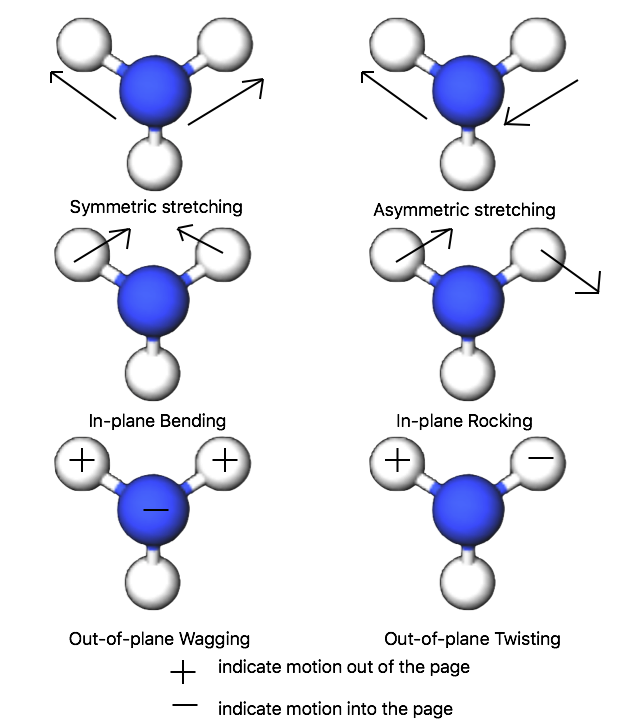
\includegraphics[width=\textwidth]{figures/chapter2/vibration.png}
\caption{Different vibrational modes of a three atom molecule.}
\label{fig:vibration}
\end{figure}

By Beer’s Law, we may calculate the column density of the molecule with its functional groups, which are used to plot figures in chapter 3 and 4. Beer Lambert’s Law suggest that when light passes through a medium, amount of light absorbed is proportional to density and path length of the medium. Assume the known intensity beam $I_{0}(\nu)$ passes through the medium and beam intensity become $I(\nu)$. The transmittance $T(\nu)$ is defined by equation \ref{eq:transmittance}. \\
\begin{equation}
T(\nu) = \frac{I(\nu)}{I_{0}(\nu)}
\label{eq:transmittance}
\end{equation}
Also, the absorbance $a(\nu)$ is defined by equation \ref{eq:absorbance}. \\
\begin{equation}
a(\nu) = - \ln T(\nu) = - \ln \frac{I(\nu)}{I_{0}(\nu)} = n l \sigma(\nu)
\label{eq:absorbance}
\end{equation}
where $n$ is number density (molecules/cm$^3$), $l$ is the path length (cm), $\sigma(\nu)$ is the cross-section (cm$^2$/molecule) of corresponding frequency $\nu$. This equation is known as Lambert Beer’s Law. \\

As the ice mixture in our thesis are at 14K, the peaks of absorbance are often a broadband due to coupling between neighbor molecules. Therefore, we can integrate the whole band of the peak equation \ref{eq:absorbance} with respect to frequency and use the absorbance strength (A value) in literatures to calculate the column densities $N$ of the ices by equation \ref{eq:column_density}.

\begin{equation}
N = \frac{\int a(\nu) \mathrm{d}\nu}{A(\nu)}
\label{eq:column_density}
\end{equation}
where $N$ is the column density (molecule cm$^{-2}$), $A(\nu)$ is the absorbance strength (cm molecule$^{-1}$).

\section{Reaction Rate Laws}
\label{sec:Reaction_Rate_Laws}
In this section, we will introduce rate reaction of a consecutive reaction and the concept of pseudo first order which we used to fit our reaction product against irradiation time. The rate of a chemical reaction is the relation between change in concentration of a substance per unit of time. i.e. For a balanced chemical reaction, A $\rightarrow$ 2B, the rate of reaction is $- \frac{\Delta [A]}{\Delta t}$. The formation rate of B is 2 times destruction rate of A.

When there are two reactants, with balanced equation 2A + B $\rightarrow$ 2C. The reaction is a third order overall, second order in A and first order in B. rate $ = k [A]^2 [B]$.

To determine the order of a reaction, we can only determine it experimentally. One way is method of initial rates. By changing concentration of initial reactants, and find out the initial reaction rate, we may find out the relation between two reactants and the rate. i.e. rate $ = k [A]^x [B]^y $.
For a reaction with only one reactant $[R]$, we may use the relation between time and reactant concentration to plot graphs to find out the order or reaction.
For a zero order reaction, the rate is not depending on any reactant that it is a constant. The rate $ = - \frac{\Delta [R]}{\Delta t} = k[R]^0$. By calculus, $[R]_0 - [R]_t = kt$.

For a first order reaction, rate $ = - \frac{\Delta [R]}{\Delta t} = k[R]$. By calculus, $\ln [R]_t = -kt + \ln [R]_0$.

For a second order reaction, rate $ = - \frac{\Delta [R]}{\Delta t} = k[R]^2$. By calculus, $\frac{1}{[R]_t} - \frac{1}{[R]_0} = kt$.

Hence, if we get a straight line in a plot between time as x-axis, and the concentration of reactant as y axis, it is a zeroth order reaction, similarly, in first order reactions, we get straight line in plots between $\ln [R]$ as y axis and t in x axis.

In a reaction with one reactant in excess, the rate of reaction is called pseudo first order reaction where pseudo means pretended. For A+B $\rightarrow$ C, rate $ = k[A][B]$. As $[B]_0 \gg [A]_0$, change of $[B]$ is negligible that $[B] \sim [B]_0$. Therefore, $[B]$ is assumed to be a constant and included in the rate constant k.

For a consecutive reaction, where A $\rightarrow$ B $\rightarrow$ C that the produced product will not convert back as reactant. A simple example is radioactive decay. At $t=0$, $[A]=[A]_0$, $[B]=0$, $[C]=0$ and at all times, $[A]+[B]+[C]=[A]_0$. The rate equations are as follows:
\begin{equation}
- \frac{\Delta [A]}{\Delta t} = k_1 [A]
\label{eq:rate1}
\end{equation}

\begin{equation}
- \frac{\Delta [B]}{\Delta t} = k_1 [A] - k_2 [B]
\label{eq:rate2}
\end{equation}

\begin{equation}
- \frac{\Delta [C]}{\Delta t} = k_2 [B]
\label{eq:rate3}
\end{equation}
By equation \ref{eq:rate1}, we get
\begin{equation}
[A] = [A]_0 e^{-k_1 t}
\label{eq:rate4}
\end{equation}
By substituting equation \ref{eq:rate4} into equation \ref{eq:rate2}, we get

\begin{equation}
- \frac{\Delta [B]}{\Delta t} + k_2 [B] = k_1 [A]_0 e^{-k_1 t}
\label{eq:rate5}
\end{equation}
After solving the differential equation \ref{eq:rate5} , we get
\begin{equation}
[B] = \frac{k_1}{k_2 - k_1} (e^{-k_1 t} - e^{-k_2 t}) [A]_0
\label{eq:rate6}
\end{equation}
Finally, since $[C]=[A]_0 -[B]-[A]$, by equation \ref{eq:rate4} and \ref{eq:rate6}, we get
\begin{equation}
[C] = \Bigg( 1+ \frac{k_1 e^{-k_2 t} - k_2 e^{-k_1 t}}{k_2 - k_1} \Bigg) [A]_0
\label{eq:rate7}
\end{equation}
